\let\negmedspace\undefined
\let\negthickspace\undefined
\documentclass[journal]{IEEEtran}
\usepackage[a5paper, margin=10mm, onecolumn]{geometry}
\usepackage{lmodern} % Ensure lmodern is loaded for pdflatex
\usepackage{tfrupee} % Include tfrupee package

\setlength{\headheight}{1cm} % Set the height of the header box
\setlength{\headsep}{0mm}     % Set the distance between the header box and the top of the text

\usepackage{gvv-book}
\usepackage{gvv}
\usepackage{cite}
\usepackage{amsmath,amssymb,amsfonts,amsthm}
\usepackage{algorithmic}
\usepackage{graphicx}
\usepackage{textcomp}
\usepackage{xcolor}
\usepackage{txfonts}
\usepackage{listings}
\usepackage{enumitem}
\usepackage{mathtools}
\usepackage{gensymb}
\usepackage{comment}
\usepackage[breaklinks=true]{hyperref}
\usepackage{tkz-euclide} 
\usepackage{listings}                                      
\def\inputGnumericTable{}                                 
\usepackage[latin1]{inputenc}                                
\usepackage{color}                                            
\usepackage{array}                                            
\usepackage{longtable}
\usepackage{multicol}
\usepackage{calc}                                             
\usepackage{multirow}                                         
\usepackage{hhline}                                           
\usepackage{ifthen}                                           
\usepackage{lscape}
\begin{document}

\bibliographystyle{IEEEtran}
\vspace{3cm}

\title{12.8.3.8}
\author{EE24BTECH11006 - Arnav Mahishi}
% \maketitle
% \newpage
% \bigskip
{\let\newpage\relax\maketitle}

\renewcommand{\thefigure}{\theenumi}
\renewcommand{\thetable}{\theenumi}
\setlength{\intextsep}{10pt} % Space between text and floats


\numberwithin{equation}{enumi}
\numberwithin{figure}{enumi}
\renewcommand{\thetable}{\theenumi}


\textbf{Question}:\newline
Find the area of the smaller region bounded by the ellipse $\frac{x^2}{9}+\frac{y^2}{4}=1$ and the line $\frac{x}{3}+\frac{y}{2}=1$
\newline
\begin{table}[h!]    
  \centering
  \begin{tabular}[10pt]{ |c| c| c|}
    \hline
    \textbf{input}&\textbf{Description}&\textbf{value}\\
    \hline 
    $a$&Length of semi major axis of ellipse&$3$\\
    \hline
    $b$&Length of semi minor axis of ellipse&$2$\\
    \hline
    $v$&Quadratic form of matrix&$\myvec{b^2&0\\0&a^2}$\\
    \hline 
    $u$&Linear coefficient vector&$0$\\
    \hline 
    $f$&Constant Term&$-(a^2b^2)$\\
    \hline
    $h$&One of the points the line passes through&$\myvec{a\\0}$\\
    \hline
    $m$&Slope of line&$\myvec{\frac{1}{b}\\\frac{-1}{a}}$\\
    \hline
    $n$& number of subintervals we are taking & $1000$\\
    \hline
    $x_0$&$x$ coordinate of first intersection point& $3$\\
    \hline
    $x_n$& $y$ coordinate of second intersection point& $2$\\
    \hline
    \end{tabular}

  \caption{Variables Used}
  \label{tab1.1.2.2}
\end{table}
\newline
Theoretical Solution:\\
The point of intersection of the line with the ellipse is $x_i=h+k_i m$,\\
where,$k_i$ is a constant and is calculated as follows:-
$$k_i=\frac{1}{m^\top Vm}\brak{-m^\top \brak{Vh+u}\pm \sqrt{\sbrak{m^\top \brak{Vh+u}}^2-g\brak{h}\brak{m^\top Vm}}}$$\\
Substituting the input parameters in $k_i$,\\
\begin{multline}
     k_i =\frac{1}{\myvec{\frac{1}{b}&\frac{-1}{a}}\myvec{b^2&0\\0&a^2}\myvec{\frac{1}{b}\\\frac{-1}{a}}}\brak{-\myvec{\frac{1}{b}&\frac{-1}{a}}\brak{\myvec{b^2&0\\0&a^2}\myvec{a\\0}+\myvec{0\\0}}\pm \\
     \sqrt{\sbrak{\myvec{\frac{1}{b}&\frac{-1}{a}}\brak{\myvec{b^2&0\\0&a^2}\myvec{a\\0}+\myvec{0\\0}}}^2-g\brak{h}\brak{\myvec{\frac{1}{b}&\frac{-1}{a}}\myvec{b^2&0\\0&a^2}\myvec{\frac{1}{b}\\\frac{-1}{a}}}}} 
\end{multline}
We get,\\
$$k_i= 0,-ab$$
Substituting $k_i$ in $x_i=h+k_i m$  we get,\\
\begin{align}
     x_1&=\myvec{a\\0}+\brak{0}\myvec{\frac{1}{b}\\\frac{-1}{a}}\\
    \implies x_1 &=\myvec{a\\0}\\
    x_2 &=\myvec{a\\0}+\brak{-ab}\myvec{\frac{1}{b}\\\frac{-1}{a}}\\
    \implies x_2&=\myvec{a\\0}+\myvec{-a\\b}\\
    \implies x_2&=\myvec{0\\b}
\end{align}
The area of the smaller region bounded by the ellipse $\frac{x^2}{9}+\frac{y^2}{4}=1$ and the line $\frac{x}{3}+\frac{y}{2}=1$ is
\begin{align}
    &=\int_{0}^{a} \frac{b}{a}\sqrt{a^2-x^2} \,dx-\int_{0}^{a} \frac{b}{a}\brak{a-x} \,dx\\
    &=\frac{b}{a}\brak{\frac{x}{2}\sqrt{a^2-x^2}+\frac{a^2}{2}\sin^{-1}{\frac{x}{a}}-ax+\frac{x^2}{2}}\limits_{0}^{a}\\
    &=\frac{b}{a}\brak{\frac{\pi a^2}{4}-\frac{a^2}{2}}=\frac{ab}{2}\brak{\frac{\pi}{2}-1}
\end{align}
The given area is $\frac{ab}{2}\brak{\frac{\pi}{2}-1}$ sq. units\\
$\therefore$ Upon substituting $a=3,b=2$ the given area is $3\brak{\frac{\pi}{2}-1}\text{sq. units}\approx1.712$ sq. units\\
\newline
Computational Solution:\\
Using the Trapezoidal rule which approximates the integral of a function $f\brak{x}$ over an interval $\sbrak{a,b}$ by dividing the interval into $n$ subintervals and approximating the area under the curve as a series of trapezoids
\begin{align}
    \int_a^b f\brak{x}dx\approx\frac{h}{2}\sbrak{f\brak{x_0}+2\sum_{i=1}^{n-1}f\brak{x_i}+f\brak{x_n}}
\end{align}
Where $x_0$ is semi-major axis of ellipse and $x_n$ is semi-minor axis of the ellipse and $h$ is the width of each subinterval.
\begin{align}
    x_i=x_0+i\cdot h\\
    h=\frac{b-a}{n}
\end{align}
In the case of our problem of the area between the line and ellipse the area is computed by:
\begin{align}
    A=\int_{x_{start}}^{x_{end}}\brak{f_{ellipse}\brak{x}-f_{line}\brak{x}}dx\\
    f_{ellipse}\brak{x}=\sqrt{4\brak{1-\frac{x^2}{9}}}\\
    f_{line}\brak{x}=2-\frac{2x}{3}
\end{align}
Where $\sbrak{x_{start},x_{end}}$ are the intersection points. Using the difference equation which iteratively computes the integral by adding the contributions of each subinterval. Let $A_k$ represent the area approximation after $k$ subintervals:
\begin{align}
    A_k&=A_{k-1}+\frac{h}{2}\sbrak{f\brak{x_k}+f\brak{x_{k-1}}}\\
    x_k&=x_{start}+k\cdot h\\
    \implies A_k&=A_{k-1}+\frac{h}{2}\sbrak{\brak{f_{ellipse}\brak{x_n}-f_{line}\brak{x_k}}+\brak{f_{ellipse}\brak{x_{k-1}}-f_{line}\brak{x_{k-1}}}}
\end{align}
Start with $A_0=0$ then iteratively calculate $f_{ellipse}\brak{x_i}$ and $f_{line}\brak{x_{i}}$ for each i from $x_{start}$ to $x_{end}$ and calculate each $A_k$ from $0$ to $n$. The value of $A_n$ will be the approximate area of the ellipse. As $n$ tends to infinity $A_n$ will be the exact area of the ellipse.
\begin{figure}[h!]
   \centering
   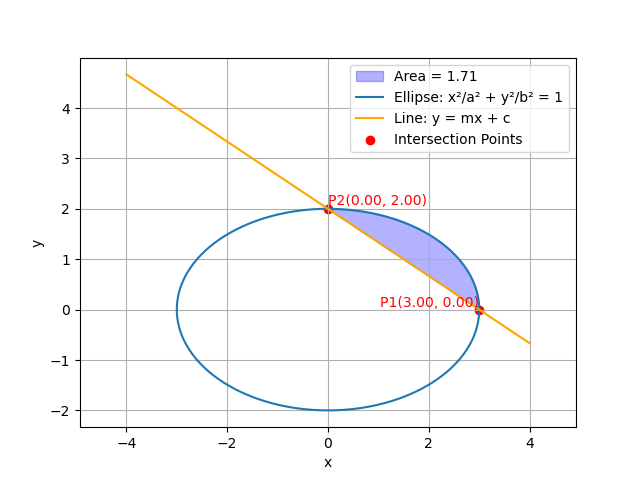
\includegraphics[width=1\linewidth]{figs/fig.png}
   \caption{Plot of area enclosed between the line and ellipse}
   \label{stemplot}
\end{figure}
\end{document}
